\iffalse
\let\negmedspace\undefined
\let\negthickspace\undefined
\documentclass[journal,12pt,twocolumn]{IEEEtran}
\usepackage{cite}
\usepackage{amsmath,amssymb,amsfonts,amsthm}
\usepackage{algorithmic}
\usepackage{graphicx}
\usepackage{textcomp}
\usepackage{xcolor}
\usepackage{txfonts}
\usepackage{listings}
\usepackage{enumitem}
\usepackage{mathtools}
\usepackage{gensymb}
\usepackage{comment}
\usepackage[breaklinks=true]{hyperref}
\usepackage{tkz-euclide} 
\usepackage{listings}
\usepackage{gvv}                                        
%\def\inputGnumericTable{}                                 
\usepackage[latin1]{inputenc}                                
\usepackage{color}                                            
\usepackage{array}                                            
\usepackage{longtable}                                       
\usepackage{calc}                                             
\usepackage{multirow}                                         
\usepackage{hhline}                                           
\usepackage{ifthen}                                           
\usepackage{lscape}
\usepackage{tabularx}
\usepackage{array}
\usepackage{float}


\newtheorem{theorem}{Theorem}[section]
\newtheorem{problem}{Problem}
\newtheorem{proposition}{Proposition}[section]
\newtheorem{lemma}{Lemma}[section]
\newtheorem{corollary}[theorem]{Corollary}
\newtheorem{example}{Example}[section]
\newtheorem{definition}[problem]{Definition}
\newcommand{\BEQA}{\begin{eqnarray}}
\newcommand{\EEQA}{\end{eqnarray}}
\newcommand{\define}{\stackrel{\triangle}{=}}
\theoremstyle{remark}
\newtheorem{rem}{Remark}
\begin{document}

\bibliographystyle{IEEEtran}
\vspace{3cm}

\title{11.9.3.17}
\author{EE23BTECH11017 - Eachempati Mihir Divyansh$^{*}$% <-this % stops a space
}
\maketitle
\newpage
\bigskip

\renewcommand{\thefigure}{\theenumi}
\renewcommand{\thetable}{\theenumi}

\textbf{Question: }
If the $4^{th}$, $10^{th}$ and $16^{th}$ terms of a G.P. are $x$, $y$, and $z$, respectively. Prove that $x,\; y,\; z$ are in G.P.
\\
\solution
\fi
\begin{table}[h]
    \centering
        \input{2023/EE/"wrong assignment"/tables/Table.tex}\label{tab: 1}
                \caption{\textbf{Given Information}}
\end{table} 
\begin{enumerate}
\item From \tabref{tab: 1},
\begin{align}
    x&= x\brak{3} =x\brak{0}r^3 \\
	y&=x\brak{9}=x\brak{0}r^{9} \\
	z&=x\brak{15}=x\brak{0}r^{15}
\end{align}
Consider $\frac{x\brak{9}}{x\brak{3}}$ and $\frac{x\brak{15}}{x\brak{9}}$;
\begin{align}
	\frac{x\brak{9}}{x\brak{3}} &= \frac{x\brak{0}r^{9}}{x\brak{0}r^3} = r^6 = \frac{x\brak{15}}{x\brak{9}} = \frac{x\brak{0}r^{15}}{x\brak{0}r^{9}}\label{eqn: 4}
\end{align}
From \eqref{eqn: 4}, $x\brak{3}$, $x\brak{9}$, $x\brak{15}$ are in G.P.\\
$\therefore$  $x$, $y$, $z$ are in G.P.\\

\item
$x\brak{0}$ and $r$ can be expressed in terms of $x$, $y$, and $z$ in the following manner.
\begin{align}
    &\frac{y}{x}=r^6 \\
	\implies& r=\sqrt[6]{\frac{y}{x}}=\brak{\frac{y}{x}}^{\frac{1}{6}}\\
    \implies& x\brak{0}=\frac{x}{r^3} =x\brak{\frac{x}{y}}^{\frac{3}{6}}\\
	\therefore\; x\brak{0}&=x^{\frac{5}{3}}y^{-\frac{2}{3}}\;
	\text{and}\; r=\brak{\frac{y}{x}}^{\frac{1}{6}}= y^{\frac{1}{6}}x^{-\frac{1}{6}} \label{eqn: 8}
\end{align}
\item 
From \eqref{eq:gpz} Z-transform of a G.P. is
\begin{align}
    X\brak{z}&=\frac{x\brak{0}}{1-rz^{-1}}; \abs{z}>\abs{r}
\end{align}
Substituting $r$ and $x\brak{0}$ from \eqref{eqn: 8}, 
\begin{align}
     X\brak{z}&=\frac{x^{\frac{5}{3}}y^{-\frac{2}{3}}}{1-{\brak{\frac{y}{x}}^{\frac{1}{6}}}z^{-1}}
\end{align}
\item Example 
Let $x(0)=1$ and $r=1.2$
\begin{align}
    x=x\brak{3}=& \brak{1.2}^3 \\
    y=x\brak{9}=&=\brak{1.2}^9\\
    z=x\brak{15}=&\brak{1.2}^{15}
\end{align}
\begin{figure}[h]
    \renewcommand\thefigure{1}
    \centering
    \caption{Stem Plot of $x(n)$ v/s $n$}
   % \caption{Stem Plot of $x(n)$ vs $n$}
    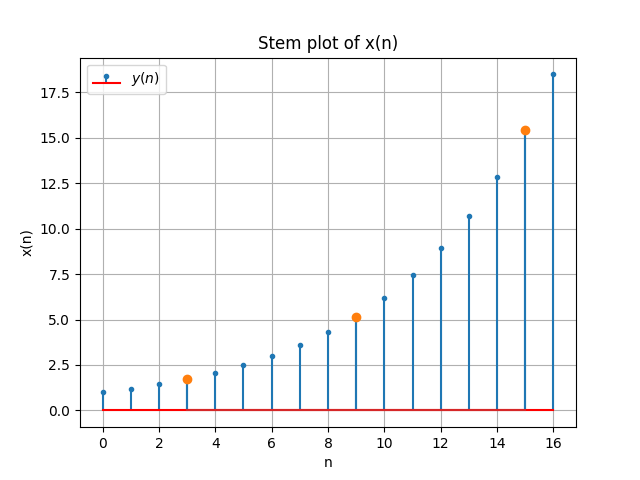
\includegraphics[width=\columnwidth]{2023/EE/"wrong assignment"/figs/A_1.png}
        \label{fig:1}
\end{figure}


\end{enumerate}
